\documentclass[a4paper]{article}

\input{style/ch_xelatex.tex}
\input{style/scala.tex}

%代码段设置
\lstset{numbers=left,
basicstyle=\tiny,
numberstyle=\tiny,
keywordstyle=\color{blue!70},
commentstyle=\color{red!50!green!50!blue!50},
frame=single, rulesepcolor=\color{red!20!green!20!blue!20},
escapeinside=``
}

\graphicspath{ {images/} }
\usepackage{ctex}
\usepackage{graphicx}
\usepackage{color,framed}%文本框
\usepackage{listings}
\usepackage{caption}
\usepackage{amssymb}
\usepackage{enumerate}
\usepackage{xcolor}
\usepackage{bm} 
\usepackage{lastpage}%获得总页数
\usepackage{fancyhdr}
\usepackage{tabularx}  
\usepackage{geometry}
\usepackage{minted}
\usepackage{graphics}
\usepackage{subfigure}
\usepackage{float}
\usepackage{pdfpages}
\usepackage{pgfplots}
\pgfplotsset{width=10cm,compat=1.9}
\usepackage{multirow}
\usepackage{footnote}
\usepackage{booktabs}

%-----------------------伪代码------------------
\usepackage{algorithm}  
\usepackage{algorithmicx}  
\usepackage{algpseudocode}  
\floatname{algorithm}{Algorithm}  
\renewcommand{\algorithmicrequire}{\textbf{Input:}}  
\renewcommand{\algorithmicensure}{\textbf{Output:}} 
\usepackage{lipsum}  
\makeatletter
\newenvironment{breakablealgorithm}
  {% \begin{breakablealgorithm}
  \begin{center}
     \refstepcounter{algorithm}% New algorithm
     \hrule height.8pt depth0pt \kern2pt% \@fs@pre for \@fs@ruled
     \renewcommand{\caption}[2][\relax]{% Make a new \caption
      {\raggedright\textbf{\ALG@name~\thealgorithm} ##2\par}%
      \ifx\relax##1\relax % #1 is \relax
         \addcontentsline{loa}{algorithm}{\protect\numberline{\thealgorithm}##2}%
      \else % #1 is not \relax
         \addcontentsline{loa}{algorithm}{\protect\numberline{\thealgorithm}##1}%
      \fi
      \kern2pt\hrule\kern2pt
     }
  }{% \end{breakablealgorithm}
     \kern2pt\hrule\relax% \@fs@post for \@fs@ruled
  \end{center}
  }
\makeatother
%------------------------代码-------------------
\usepackage{xcolor} 
\usepackage{listings} 
\lstset{ 
breaklines,%自动换行
basicstyle=\small,
escapeinside=``,
keywordstyle=\color{ blue!70} \bfseries,
commentstyle=\color{red!50!green!50!blue!50},% 
stringstyle=\ttfamily,% 
extendedchars=false,% 
linewidth=\textwidth,% 
numbers=left,% 
numberstyle=\tiny \color{blue!50},% 
frame=trbl% 
rulesepcolor= \color{ red!20!green!20!blue!20} 
}

%-------------------------页面边距--------------
\geometry{a4paper,left=2.3cm,right=2.3cm,top=2.7cm,bottom=2.7cm}
%-------------------------页眉页脚--------------
\usepackage{fancyhdr}
\pagestyle{fancy}
\lhead{\kaishu \leftmark}
% \chead{}
\rhead{\kaishu 并行程序设计实验报告}%加粗\bfseries 
\lfoot{}
\cfoot{\thepage}
\rfoot{}
\renewcommand{\headrulewidth}{0.1pt}  
\renewcommand{\footrulewidth}{0pt}%去掉横线
\newcommand{\HRule}{\rule{\linewidth}{0.5mm}}%标题横线
\newcommand{\HRulegrossa}{\rule{\linewidth}{1.2mm}}
\setlength{\textfloatsep}{10mm}%设置图片的前后间距
%--------------------文档内容--------------------

\begin{document}
\renewcommand{\contentsname}{目\ 录}
\renewcommand{\appendixname}{附录}
\renewcommand{\appendixpagename}{附录}
\renewcommand{\refname}{参考文献} 
\renewcommand{\figurename}{图}
\renewcommand{\tablename}{表}
\renewcommand{\today}{\number\year 年 \number\month 月 \number\day 日}

%-------------------------封面----------------
\begin{titlepage}
    \begin{center}
    
\includegraphics[width=0.8\textwidth]{NKU.png}\\[1cm]
    \vspace{20mm}
		\textbf{\huge\textbf{\kaishu{计算机学院}}}\\[0.5cm]
		\textbf{\huge{\kaishu{并行程序设计}}}\\[2.3cm]
		\textbf{\Huge\textbf{\kaishu{中国自主处理器架构发展调研报告}}}

		\vspace{\fill}
    
    % \textbf{\Large \textbf{并行程序设计期末实验报告}}\\[0.8cm]
    % \HRule \\[0.9cm]
    % \HRule \\[2.0cm]
    \centering
    \textsc{\LARGE \kaishu{姓名\ :\ 罗雅淇\ }}\\[0.5cm]
    \textsc{\LARGE \kaishu{学号\ :\ 2313483}}\\[0.5cm]
    \textsc{\LARGE \kaishu{专业\ :\ 计算机科学与技术}}\\[0.5cm]
    
    \vfill
    {\Large \today}
    \end{center}
\end{titlepage}

\renewcommand {\thefigure}{\thesection{}.\arabic{figure}}%图片按章标号
\renewcommand{\figurename}{图}
\renewcommand{\contentsname}{目录}  
\cfoot{\thepage\ of \pageref{LastPage}}%当前页 of 总页数


% 生成目录
\clearpage
\tableofcontents
\newpage

%--------------------------Title--------------------------------
\section{摘要}
在当今全球半导体产业地缘政治博弈加剧的背景下，计算力的自主可控已成为中国国家战略的核心。中国自主处理器（CPU/GPU/NPU）的发展历程，是一场从底层指令集架构（ISA）受制于人到建立自主知识产权体系、从通用微架构效法先进到针对特定算力需求进行结构创新的深刻转型。
\section{国产CPU/GPU/NPU发展历史}
2000年前后，科技部将通用CPU研制纳入863计划，龙芯、申威、飞腾三支国家队由此起步。此后，2014年中央网络安全和信息化领导小组的成立，以及信创政策的持续推进，进一步强化了核心芯片自主可控的战略地位。2019年以来美国实体清单制裁的持续升级，则彻底打断了国内企业依赖台积电先进制程的技术路径，客观上倒逼了全产业链的自主化进程。

在这一背景下，国产处理器形成了三条并行发展的技术线索：以飞腾为代表的国家队CPU路径、以华为海思鲲鹏/昇腾为代表的企业自主投入路径，以及以摩尔线程为代表的通用GPU新兴路径。
\subsection{飞腾CPU：从SPARC到ARM的架构迁移}
业界两大CPU技术体系分别为X86和ARM，今年来国产CPU大多选择以ARM为基础进行研发。飞腾（Phytium）的技术渊源可追溯至早期的SPARC架构探索，但其真正的跨越式发展其实是始于2014年转向ARM架构授权。

飞腾早期产品兼容SPARC v9指令集。2011年推出的FT-1500采用台积电40nm制程，应用于天河一号A的服务节点。这一阶段的价值主要在于积累完整的CPU设计、验证与物理实现能力，但是受限于SPARC架构的软件生态。

2014年飞腾转型采用ARMv8架构级授权，即在ARM指令集框架内自主设计微架构核（FTC66x系列），而非使用ARM公版Cortex核。
2019年的FT-2000/4（FTC663核）主频提升至2.6—3.0 GHz，性能相比上代翻倍，功耗降低约三分之一，并首次集成飞腾自定义的PSPA安全架构。2020年推出的8核FTC663，被广泛应用于D2000等桌面级和工业级芯片中，进一步将SPECint基准分值提升近一倍，同年腾云S2500（64核）量产，补齐高端服务器产品线。
由于国内IT产业尚无实力构建全自主软硬件生态，飞腾CPU指令集从IA-64、SPARC最终变迁到ARM，目标是为了获得更好的软件生态，这也是兼顾自主可控与实用性的一条非常好的现实路径。

\subsection{华为鲲鹏与昇腾：制裁前后的两段历史}
\subsubsection{制裁前（2004—2020）：积累阶段}
华为海思自2004年起投入CPU研发，历经Hi1610/Hi1612/Hi1616等服务器CPU迭代，于2019年1月推出旗舰产品鲲鹏920。该芯片采用台积电7nm制程，最多64核，自研TaiShan V110核（ARMv8架构级授权），集成8通道DDR4与PCIe 4.0，SPECint评分超过930分。同年，在AI加速器方向上，昇腾910（台积电7nm代工）首次亮相，昇腾属于专用集成集成电路架构的NPU（Neural Processing Unit， 神经网络处理器），专为处理神经网络计算任务设计。它是基于华为原创的“达芬奇架构”，其核心创新在于针对矩阵乘加运算的专用三维Cube计算单元设计，相较传统GPU二维MAC阵列具有更高算力密度。
\subsubsection{制裁后（2020至今）：倒逼自主化}
然而2020年美国商务部将华为列入实体清单，台积电随即停止为华为代工先进制程芯片，昇腾910的量产渠道被切断。华为被迫转向与中芯国际合作，利用DUV光刻技术实现7nm节点量产。由中芯国际代工的第二代昇腾910B每颗芯片可激活20—25个AI核心，少于台积电代工的第一代910的30—32个，反映出中芯国际在良率与产能上仍存在制约。尽管如此，昇腾910B已大面积采用自主产线量产，国内各大互联网企业相继下达大额订单，国内AI芯片市场的国产替代率显著提升。

近年的第三代昇腾910C则采取了更务实的封装策略：将两颗910B芯片通过先进封装技术整合，而非全新架构重设计，以在保证量产稳定性的前提下提升算力规模。分析师评估其性能约达H100的80%，但芯片逻辑面积比H100大60%左右，显示出在架构效率上与国际领先水平仍有差距。2025年，华为进一步发布CloudMatrix系统，集成384颗昇腾910C，在特定集群吞吐指标上宣称可比肩NVIDIA GB200 NVL72，但功耗显著更高。

\subsection{摩尔线程MUSA：通用GPU的国产探索}
与华为针对AI算力的专用路径不同，摩尔线程选择了对标NVIDIA的全功能通用GPU路径，即同时覆盖图形渲染、AI加速、科学计算与视频编解码四大引擎。其自主研发的MUSA（元计算统一系统架构）是贯穿硬件到软件的全栈技术体系。

产品迭代经历了三代芯片：
\begin{itemize}
  \item 2022年3月首发第一代"苏堤"架构及MTT S50/S2000；同年11月推出第二代"春晓"架构，基于此推出MTT S80——国内首款支持DirectX 12的消费级游戏显卡，以及面向服务器的MTT S3000；
  \item 2023年9月发布第三代"曲院"架构，推出面向大模型训练的MTT S4000及千卡级夸娥（KUAE）智算集群。
  \item 2025年，摩尔线程进一步发布第四代"花港"架构，宣称在相同工艺条件下算力密度提升50\%，并完成科创板上市，成为国产GPU领域首家公开挂牌企业。
\end{itemize}

软件生态上，摩尔线程提供MUSIFY代码自动转换工具，支持将CUDA代码迁移至MUSA平台，同时兼容PyTorch、TensorFlow等主流深度学习框架，构建独立于CUDA之外的国产GPU软件栈。

\subsection{总结：三条技术路径的共性}
观察上述的三条发展路径，可以归纳出一个共同的结构性规律：由于国产处理器发展较晚，面对当前卡脖子问题，想要弯道超车大多企业采用的策略是在硬件层面寻求架构级自主，在软件生态层面寻求与国际标准的最大兼容。比如，飞腾和鲲鹏均选择ARMv8架构级授权而非公版核，摩尔线程则通过CUDA兼容层降低软件迁移成本。但是理性地选择ARM架构授权并不以为着完全没有风险，这一授权关系本身即构成潜在的政治风险——若ARM公司迫于压力停止向中国企业续签架构级授权，国产CPU的技术路线将面临根本性动摇。

正是在这一背景下，RISC-V作为一种完全开源、无需授权费的指令集架构，则成为指令集层面实现彻底自主的战略备选。香山处理器项目就是在RISC-V路线上进行发展的，经历了雁栖湖、南湖、昆明湖三代演进，第三代"昆明湖（KMH）“核心采用6发射乱序超标量架构，支持RISC-V RVA23配置文件及向量（V）和虚拟化（H）扩展。据估算，在3GHz频率下SPECint2006评分可达约45分，足以与ARM Neoverse-N2一较高下。然而，虽然通过近年来的努力我国芯片设计的自主化程度已显著提升，但是先进制程代工对台积电的依赖所暴露的制造端脆弱性依然是一个尚未解决的问题。同时ARM架构授权也是一个隐藏的问题，

\section{代表性国产CPU/NPU微架构深度调研}
本报告选取鲲鹏920（通用CPU）与昇腾910（AI NPU）作为代表性对象，进行了深度的调研。

\subsection{鲲鹏920：面向云计算的通用服务器CPU}
\subsubsection{整体SoC架构}
鲲鹏920内部并不是简单的“一堆核心加一块内存”，它的核心是以“集群”（Cluster）方式组织的，采用Chiplet封装方案，由多个CPU计算芯粒与一颗16nm IO芯粒组合而成，其中：
\begin{itemize}
  \item 每颗CPU计算芯粒集成32个TaiShan V110核心，四核共享一组LLC标签，对应LLC数据分布在邻近的片上网络节点；
  \item DDR控制器两两成对组织，每个芯粒设置独立的归属代理单元（HHA）负责一致性管理；
  \item 片间通过超级集群链路层连接器（SLLC）实现带缓存一致性的跨芯粒通信。
\end{itemize}

完整的鲲鹏920服务器版本由两颗芯粒组合，最终提供64核心、8通道DDR4、总内存带宽高达1.5 Tb/s，支持PCIe 4.0及CCIX接口，总带宽640 Gbps，片间通过华为缓存一致性总线（HCCS）480 Gbps互联，最多支持四颗鲲鹏920组成256核NUMA系统。
\begin{figure}[H]
  \centering
  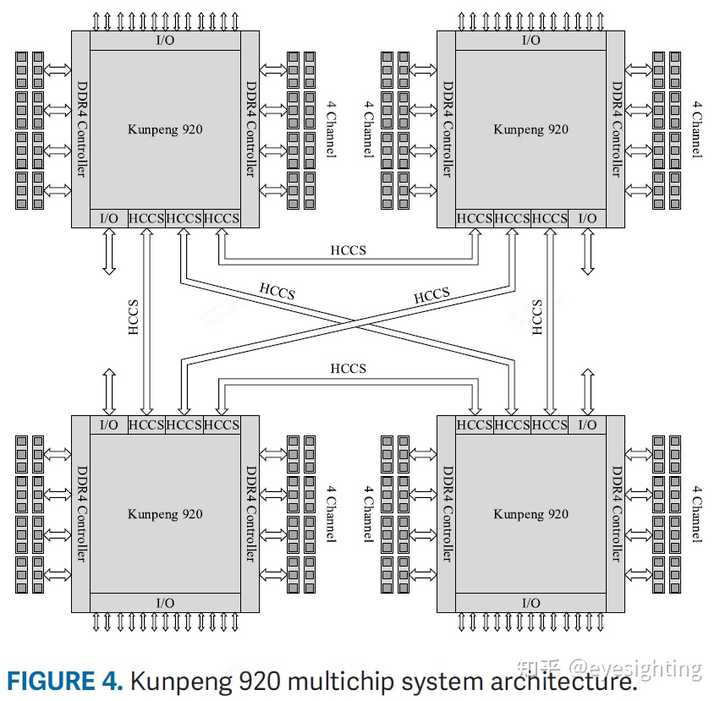
\includegraphics[width=0.65\textwidth]{fig/image2.png}
\end{figure}
这一Chiplet设计的核心意图在于将计算芯粒与IO芯粒分开制造，前者采用7nm工艺追求计算密度，后者采用16nm兼顾IO接口的工艺成熟度，同时通过模块化复用降低设计成本。这种乐高式架构允许各种芯片组合与不同封装技术无缝集成，以满足不同的工作负载要求。

\subsubsection{TaiShan V110单核微架构}
CPU 计算芯片包含三个组件：1）Taishan V110 内核； 2）末级缓存（LLC）设计； 3) 无缓冲NoC。本文主要调研了TaiShan V110的架构设计，作为华为基于ARMv8.2架构级授权自主设计的服务器核心，其微架构针对云计算典型负载，比如大数据分析、分布式存储、高并发服务，进行了定制优化。
\begin{enumerate}
  \item 前端——取值与分支预测：超标量流水线主要由取指令、指令译码、指令分派和整数执行组成。取指部件每周期最多从64 KB、4路组相联L1指令缓存中取出4条指令，分支预测单元同时支持静态与动态两种策略，动态预测通过两级预测器结合分支目标缓冲区（BTB）实现高速目标地址生成。

  经调研，独立评测揭示了TaiShan V110前端设计具有一定的局限性，其L1 BTB容量约64项，且按cache line而非block组织，当指令流中分支密度较高时有效容量会急剧下降；此外缺乏有效的指令预取机制，在代码足迹较大的负载下会出现较高的L1指令缓存失效率。这些特征表明TaiShan V110的前端设计偏保守，在大规模程序代码场景下存在明显瓶颈。
  \item 后端——乱序执行：后端执行单元包括3条整数ALU流水线、1条整数乘除法单元（MDU）、2条浮点/向量（AdvSIMD）执行流水线，以及2个Load/Store端口并集成硬件自动预取器。乱序执行窗口在当时规模较大，Load Queue容量48项，Store Queue容量32项，与执行单元规格（2个Load AGU、1个Store AGU）相匹配。
  
\end{enumerate}

\subsubsection{存储层级与片上互联}
鲲鹏920实现了多级内存层次结构。主要目的是将经常使用的数据子集放置在更靠近 CPU 核心的位置，以便更有效地管理加载/存储。下表列出了预期的带宽和延迟参数，并说明了它们在每个内存级别之间变化的平滑程度。两级互连（包括芯片间和芯片间连接）经过精心设计，以最大程度地减少存储器层次结构各级中不必要的数据移动。

\subsection{昇腾910：面向AI训练的专用NPU}

\subsubsection{整体架构}
神经网络训练的计算核心是海量的矩阵乘加运算，传统的GPU通过CUDA核心阵列和Tensor Core来加速这一过程，而昇腾910的设计理念是更进一步：将矩阵计算从二维MAC阵列升维至三维Cube结构，在硅片面积上以更高密度执行矩阵运算。

昇腾910 SoC集成32个DaVinci AI Core（用于神经网络计算）与4个AI CPU核心（基于TaiShan架构，负责非矩阵的通用控制计算），所有组件通过内部总线互联。32个DaVinci核在片上以6行4列的Mesh片上网络（NoC）拓扑排列，采用台积电7nm+ EUV工艺，峰值算力FP16达256 TFLOPS，INT8达512 TOPS，功耗约310 W；IO功能由独立的Nimbus V3芯片承担，与主芯片及HBM2通过硅中介层共封装。

\begin{figure}[H]
  \centering
  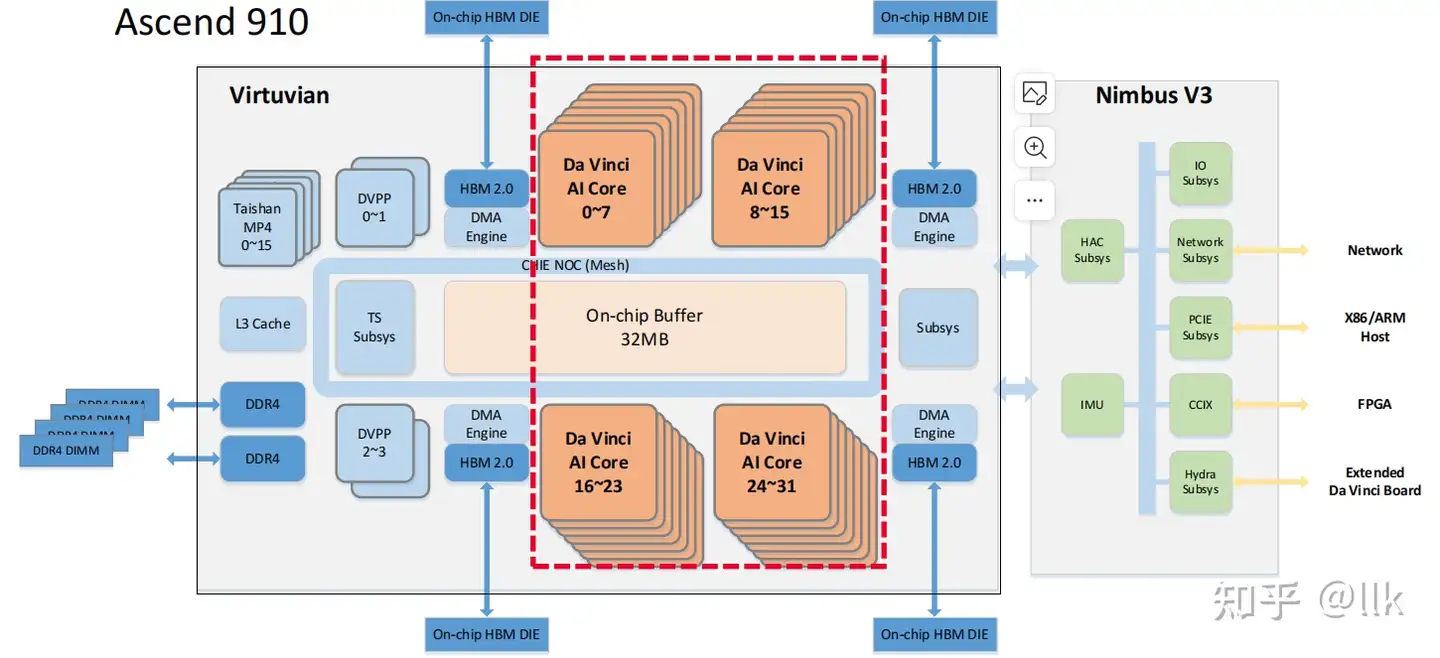
\includegraphics[width=0.8\textwidth]{fig/image1.png}
\end{figure}

\subsubsection{DaVinci Core：三维计算单元的设计逻辑}
DaVinci Core是达芬奇架构的基本计算单元，也是昇腾的创新核心，它针对神经网络计算模式设计的三类计算单元协同工作机制。分别是：
\begin{itemize}
  \item Cube单元（矩阵计算）：卷积层、全连接层等线性运算（占神经网络计算量85\%以上）由Cube单元承担；
  \item Vector单元（向量计算）：激活函数、归一化等逐元素非线性运算由Vector单元承担；
  \item Scalar单元（标量控制）：循环控制与地址计算由Scalar单元承担。
\end{itemize}

\subsubsection{片上存储层级}
AI芯片面临还有一个矛盾是Cube单元产生算力的速度远超HBM供应数据的速度，内存带宽成为制约训练效率的主要瓶颈，即"内存墙"问题。达芬奇架构通过多层次片上缓冲体系来缓解这一矛盾。

每个DaVinci Core内部设有L0 Buffer，直接为Cube/Vector单元供料，访问延迟最低；多个Core共享L1 Buffer，用于复用跨核的激活值；整个SoC设有L2 Cache作为片上最后一级缓存，片上NoC以1024位宽、2 GHz时钟连接各DaVinci Core，提供对片上L2缓存4 TB/s的访问带宽与对HBM2 1.2 TB/s的访问带宽。
\begin{figure}[H]
  \centering
  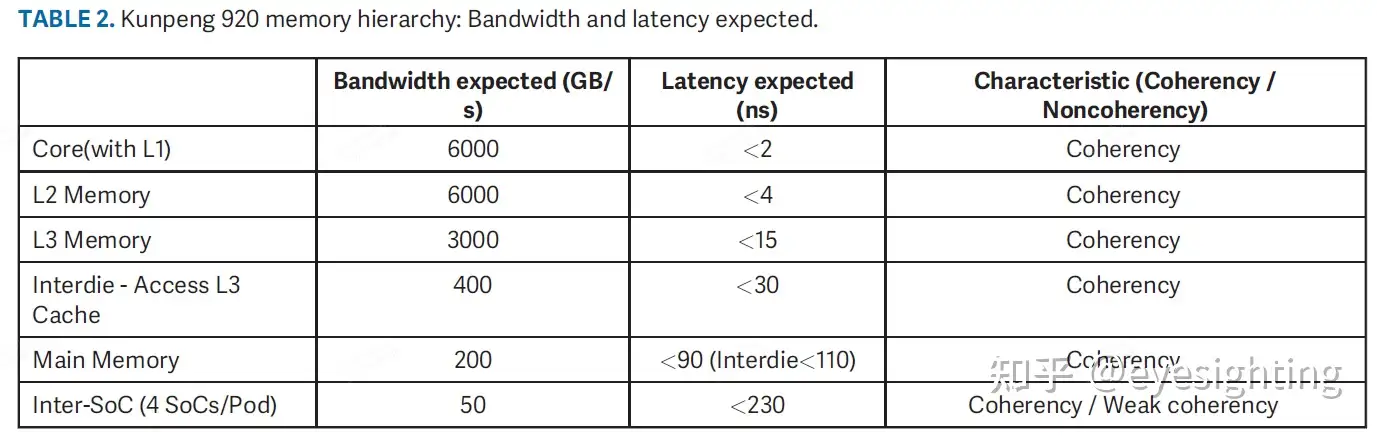
\includegraphics[width=1\textwidth]{fig/image3.png}
\end{figure}

这种设计的本质是通过软件策略将神经网络层切分为适合L0/L1 Buffer大小的计算块（tile），使Cube单元尽可能在片上缓冲命中的状态下持续工作，将HBM访问隐藏在计算延迟背后。这也是为何昇腾的编程模型与CUDA有根本差异——CUDA对程序员屏蔽了显式的缓存管理，而CANN中的算子开发需要程序员或编译器显式控制各级Buffer的数据搬运。



\section{进阶调研：国内外最新处理器对比}

% --- 正文开始 ---

\subsection{桌面CPU横向对比：以飞腾为基准}

\subsubsection{国内外最新桌面CPU参数对比}



\begin{table}[H]
\centering
\caption{桌面CPU横向对比——以飞腾为基准}
\small
\begin{tabularx}{\textwidth}{lXXXX}
\toprule
\textbf{对比维度} & \textbf{飞腾腾锐D3000} & \textbf{Intel Core Ultra 9 285K} & \textbf{AMD Ryzen 9 9950X} & \textbf{Apple M5 Pro} \\
\midrule
定位 & 国产信创桌面 & 消费级高端桌面 & 消费级旗舰桌面 & 专业移动端处理器 \\
核心 & 8核 FTC862 & 24核 (8P+16E) & 16核 Zen5 (全大核) & 14核 (6超级+8高效) \\
制程工艺 & 约14nm (估算) & 台积电 3nm (P核) & 台积电 4nm & 台积电 3nm \\
最高主频 & 2.5 GHz & 5.7 GHz & 5.7 GHz & 4.6 GHz \\
L3缓存 & 8 MB + 8 MB L4 & 36 MB & 64 MB & 36 MB (统一) \\
内存支持 & DDR5-5600 & DDR5-6400 & DDR5-5600 & LPDDR5X 统一内存 \\
TDP & 70 W & 125 W & 170 W & $\approx$ 30 W \\
AI加速 & 无独立NPU & NPU 13 TOPS & 无独立NPU & Neural Engine 38 TOPS \\
发布时间 & 2024年6月 & 2024年10月 & 2024年7月 & 2025年 \\
实测性能 & $\approx$ Intel 10代 i5 & IPC领先13代约9\% & 单核领先Intel约10\% & 能效比领先x86平台 \\
\bottomrule
\end{tabularx}
\label{tab:cpu_comparison}
\end{table}

\subsubsection{桌面CPU差距分析与制约因素}

\textbf{制程代差：} 国际主流桌面CPU在2024年已全面迈入台积电3—4nm节点，而飞腾受制裁影响无法使用台积电先进制程，只能依赖中芯国际14nm工艺。制程落后约三代，直接导致在相同功耗预算（70W）下，可容纳的晶体管数量、可实现的主频上限均受到严格约束。即便微架构设计水平与国际相当，制程瓶颈也会将性能锁死在较低区间。

\textbf{微架构迭代速度：} Intel Arrow Lake与AMD Zen5均是历经十余代打磨的结果。飞腾FTC862核作为首代产品，在分支预测精度、执行单元数量等细节上仍有差距。同时Apple M5的案例证明，虽然同样使用ARM架构授权，但凭借超宽微架构和统一内存设计，其能效比远超x86平台，说明微架构设计深度与制程也是关键。

\subsection{GPU横向对比：以摩尔线程为基准}

\subsubsection{最新国内外GPU参数对比}

\begin{table}[H]
\centering
\caption{GPU横向对比——以摩尔线程MTT S4000为基准}
\small
\begin{tabularx}{\textwidth}{lXXXX}
\toprule
\textbf{对比维度} & \textbf{MTT S4000} & \textbf{NVIDIA H100 SXM5} & \textbf{NVIDIA B200} & \textbf{Intel Ponte Vecchio} \\
\midrule
制程工艺 & 约14/12nm (估算) & 台积电 4N & 台积电 4NP & 台积电 5nm + Intel \\
FP32算力 & 25 TFLOPS & 67 TFLOPS & $\approx$ 60 TFLOPS & 45 TFLOPS \\
FP16算力 & 100 TFLOPS & 1,979 TFLOPS & 2,250 TFLOPS & 419 TFLOPS \\
显存容量 & 48 GB GDDR6 & 80 GB HBM3 & 192 GB HBM3e & 128 GB HBM2e \\
显存带宽 & 768 GB/s & 3,350 GB/s & 8,000 GB/s & 3,276 GB/s \\
互联带宽 & 240 GB/s & 900 GB/s & 1,800 GB/s & 348 GB/s \\
软件生态 & MUSA (含转换工具) & CUDA (30年积累) & CUDA (兼容) & oneAPI / OpenCL \\
\bottomrule
\end{tabularx}
\end{table}

\subsubsection{GPU差距分析与制约因素}

MTT S4000与H100之间FP16算力高达约20倍的差距，反映了两个核心制约维度：

\textbf{显存技术瓶颈：}S4000采用GDDR6，而H100采用HBM3，带宽差距达4.4倍。大模型任务对带宽高度敏感，国内尚不具备HBM大规模量产及CoWoS先进封装能力，这是供应链层面的硬制约。

\textbf{片间互联与扩展性：} MTLink 1.0与NVLink5带宽相差数倍，导致在千卡级集群中通信效率低下，难以承接超大规模训练。

\subsection{NPU：以华为昇腾910C为基准}

\subsubsection{最新国际AI加速器（NPU）横向对比}

\begin{table}[H]
\centering
\caption{最新国际AI加速器（NPU）横向对比——以昇腾910C为基准}
\small
\begin{tabularx}{\textwidth}{lXXXX}
\toprule
\textbf{对比维度} & \textbf{昇腾910C (华为)} & \textbf{NVIDIA H100} & \textbf{NVIDIA B200} & \textbf{Google TPU v5e} \\
\midrule
制程工艺 & 中芯 7nm (N+2) & 台积电 4N & 台积电 4NP & 台积电 7nm \\
FP16算力 & $\approx$ 800 TFLOPS & 989 TFLOPS & 2,250 TFLOPS & $\approx$ 197 TFLOPS \\
显存带宽 & $\approx$ 3.2 TB/s & 3.35 TB/s & 8.0 TB/s & 819 GB/s \\
芯片面积 & H100的约160\% & 基准 (100\%) & 未披露 & 未披露 \\
单卡成本 & $\approx$ \$1,800 & $\approx$ \$30,000+ & $\approx$ \$40,000+ & 内部使用 \\
软件栈 & CANN + MindSpore & CUDA + cuDNN & CUDA & JAX / XLA \\
\bottomrule
\end{tabularx}
\end{table}

\subsubsection{NPU差距分析}

\textbf{硬件层面：} 昇腾910C通过双Die合封，以1.6倍于H100的面积代价，实现了其80\%的性能。这是在制程落后两代（中芯7nm对比台积电4N）情况下的无奈选择。此外，HBM存储器仍高度依赖外部供应链，是自主可控中最薄弱的一环。

\textbf{软件层面：} CUDA形成了三重锁定：深度调优的算子库、与框架的深度耦合、以及全球开发者的技能惯性。即便如Google TPU般投入巨大，在CUDA的生态壁垒面前也只能寻求差异化竞争。

% --- 结束 ---

\section{展望：国产处理器的突围路径}
国产处理器在外部制裁与自主战略的“双重驱动”下，正经历从指令集受制于人向建立独立知识产权体系的深刻转型。目前已形成以飞腾、鲲鹏为代表的通用CPU，以昇腾为代表的专用NPU，以及以摩尔线程为代表的全功能GPU三条核心技术路径。
\subsection{展望未来}
\begin{enumerate}
  \item 架构突围： 随着摩尔定律放缓，依靠制程缩减带来的红利递减，国产处理器将深度押注“以架构换性能”。通过Chiplet技术整合计算与IO芯粒，利用先进封装对冲制造劣势。
  \item 生态易帜： 面对ARM授权风险与CUDA壁垒，RISC-V架构（如香山项目）将成为实现指令集层面彻底自主的战略备选，通过开源生态构建新的软硬件话语权。
  \item 全栈自主： 未来突围的关键不再仅限于芯片设计，而在于国产光刻机（制造）、HBM存储器（供应链）以及CANN/MUSA等软件栈（生态）的垂直整合。国产处理器有望在AI算力与信创市场率先实现闭环，并最终在多元算力时代建立起独立于外部限制的技术范式。
\end{enumerate}


\newpage
\bibliographystyle{plain}
\bibliography{reference.bib} 

\end{document}